\begin{appendix}
\chapter{Dynamics of density matrix.}\label{AppendixA}
\section{Schr{\"o}dinger equation.}
A particular fact about the Schr{\"o}dinger equation is that it can not be derived from any mathematical formalism, its construction is phenomenological and can be seen as a postulate of quantum mechanics.\\
The Schr{\"o}dinger equation is written as follows:
\begin{equation}
i\hbar\frac{d}{dt}\ket{\psi(t)}=\hat{H}\ket{\psi(t)} \ ;\qquad \hat{H}=\hat{H}^{\dagger}
\label{scrodingereq}
\end{equation}
Some facts about this equation are:
\begin{itemize}
\item Is linear and first order in time.
\item It is deterministic.
\item Given $\ket{\psi(t)}$ and $\hat{H}$ it fixes $\ket{\psi(t')}$ for all $-\infty <t'<\infty$
\item As the operator $\hat{H}$ is hermitian Schr{\"o}dinger the equation for $\bra{\psi(t)}$ is simply given by:
\[-i\hbar\bra{\psi(t)}=\bra{\psi}\hat{H}\]

\item It preserves the norm of $\ket{\psi(t)}$.
\vspace{.5mm}
\begin{align*}
\bra{\psi}\ket {d\psi}+\bra{ d\psi}&\ket{ \psi}=\bra{\psi}\frac{-i}{\hbar}dt \hat{H}\ket{\psi}+\bra{\hat{H}\psi}\frac{i}{\hbar}dt\ket{\psi}\\
&=\frac{-i}{\hbar}dt\left(\bra{\psi}\hat{H}\ket{\psi}-\bra{\psi}\hat{H}\ket{\psi}\right)=0
\end{align*}

\[\frac{d}{dt}\mid\psi\mid^2=\frac{d}{dt}\bra{\psi}\ket{\psi}=0 \ ; \quad\mid\psi\mid=constant\]

\end{itemize}
With these properties we can then construct the evolution of the density matrix $\rho=\ket{\psi}\bra{\psi}$, by considering the evolution of $\rho$ given by the Schr{\"o}dinger equation:
\begin{equation}
i\hbar\frac{d}{dt}\ket{\psi}\bra{\psi}=\hat{H}\ket{\psi}\bra{\psi}-\ket{\psi}\bra{\psi}\hat{H}=\left[\hat{H},\rho\right],
\label{liouville-vonnuemann}
\end{equation}
this equation is also called Liouville-von Neumann equation in the Schr{\"o}dinger picture.\\
Following the same formalism, in the Heisenberg picture we see that the evolution of an operator $\hat{A}$ is given by:
\[i\hbar\frac{d}{dt}\hat{A}_H=\left[\hat{A}_H,\hat{H}_H\right]\]
Where $\hat{A}_H=\hat{U}^{\dagger}\hat{A}\hat{U}$ with $\hat{U}$ an unitary transformation. And the average of an operator $\hat{A}$ with respect to an  of states is given by:

\begin{align}
\sum_{n}p_n\bra{\psi_n}\hat{A}\ket{\psi_n}&=\sum_n p_n \text{tr}[\bra{\psi_n}\hat{A}\ket{\psi_n}] \nonumber \\
&=\sum_n p_n\text{tr}[\hat{A}\ket{\psi_n}\bra{\psi_n}] \nonumber \\
&=\text{tr}\left[\hat{A}\sum_n p_n\ket{\psi_n}\bra{\psi_n}\right]\nonumber\\
&=\text{tr}(\hat{A}\rho) \nonumber \\
&=\braket{\hat{A}} 
\label{appendixexpectedvalue}
\end{align} 

%%%%-------- Decoherence Part----------%%%%%
\section{Decoherence.}\label{appendixAdecoherence}
From the Schr{\"o}dinger equation one knows that a way to talk about quantum dynamics is in terms of unitary transformations. If a system undergoes Hamiltonian evolution for a finite time then the evolution can be described by an unitary operator $U$. In this case $\ket{\psi}\bra{\psi}$ is mapped to $U\ket{\psi}\bra{\psi}U^{\dagger}$, and by linearity, a general density matrix $\rho$ is then mapped to $U\rho U^{\dagger}$.\\
In such wise, unitary operators correspond to reversible operations or in other words, if $U$ is valid unitary time evolution then so is $U^{\dagger}$. In terms of Hamiltonians, evolution according to $-H$ will reverse evolution according to $H$. But other quantum processes such as non unitary evolution cause an irreversible loss of information.\\
To illustrate it, let's first start understanding the concept of \textit{mixture}.Mixture refers to \\

If a state $\ket{\psi_{a}}$ has a probability $p_a$ to happen, then the density matrix is $\sum_{a}p_{a}\ket{\psi_{a}}\bra{\psi_{a}}$. But in the case we've got an ensemble of density matrices $\{(p_1,\rho_1),\ldots,(p_m,\rho_m)\}$.Then the ``average'' density matrix is\footnote{This is also called a time-independent mixture.}
\begin{equation}
\rho=\sum^{m}_{a=1}p_a\rho_a.
\label{rhoapendixA}
\end{equation}
With this in mind we can use it to model \textit{random unitary evolution}, by supposing our state experiences a random Hamiltonian. Thus the correspond mapping it results by considering that unitary $U_{a}$ occurs with probability $p_a$ for $a=1,\ldots,m$, is:
\begin{equation}
\rho\longrightarrow \sum_{a=1}^{m}p_a U_a \rho U_{a}^{\dagger}.
\label{Mapping}
\end{equation}
To understand how under this mapping we can explain the loss of coherence in simple quantum systems let's check two examples.
\subsection{Evolution of polarised light.}
Suppose we start with a density matrix
\[
\rho=
  \left( 
  {\begin{array}{cc}
   \rho_{11} & \rho_{12} \\
   \rho_{21} & \rho_{22} \\
  \end{array} }
   \right),
\]
and choose a random unitary evolution which is going to perform as follows: With probability $1-p$ the matrix $\rho$ remains invariant and with probability $p$ we perform a unitary transformation corresponding to $\hat{\sigma}_z$%\footnote{This is the case of the evolution of polarized light which is observed in the $\hat{z}$ basis.}. 
then the ensemble of unitary transformations we are working with is given by $\{(1-p,I),(p,\hat{\sigma}_z)\}$. So the density matrix is mapped to:
\begin{align*}
\rho ' &\equiv (1-p)\hat{\mathds{1}}\rho \hat{\mathds{1}}^{\dagger} + p\hat{\sigma}_z \rho \hat{\sigma}_z^{\dagger}\\[0.5cm]
&=\left(
{\begin{array}{cc}
\rho_{11} & (1-2p)\rho_{12} \\
(1-2p)\rho_{21} & \rho_{22} \\
\end{array}
}
\right).
\end{align*}
First we can see two trivial different cases:
\begin{enumerate}
\item If $p=0$, of course nothing happen and the matrix remains invariant.
\item If $p=1$, we simply get $\rho$ changes as: $\rho'=\hat{\sigma}_z \rho \hat{\sigma}_z^{\dagger}$, which is translate as an unitary transformation of the density matrix.
\end{enumerate}
One can observe that the diagonal terms remain invariant, whereas the terms off-diagonal are reduced in absolute value in consequence of $\mid1-2p\mid<1$. Thus, we see the diagonal terms correspond to the probability of outcomes we would observe being in the $\hat{z}$ basis, so, it's clear that a rotation along $\hat{z}$ would not affect the results. However, the off-diagonal terms will vanish when $p=1/2$, meaning that the polarization in $\hat{x}$ and $\hat{y}$ directions has been eliminated. A way to explain why this is happening we use the fact that  the density matrix state for a two-level system can be written using the Pauli operators as:
\begin{equation}
\rho=\frac{1}{2}\left[\hat{\mathds{1}}+x\hat{\sigma}_x+y\hat{\sigma}_y+z\hat{\sigma}_z\right].
\label{Blochapendix}
\end{equation}
Where $x,y,z$ are the averages of the Pauli operators, this is $x=\textnormal{Tr}[\hat{\sigma}_x\rho]$ etcetera.Then by using the relation between the product of these operators:
\[
\hat{\sigma}_i\hat{\sigma}_j=\delta_{ij}\hat{\mathds{1}}+i\epsilon_{ijk}\hat{\sigma}_k.
\]
We can prove that:
\[
\hat{\sigma}_z\rho\hat{\sigma}_z^{\dagger}=\rho=\frac{1}{2}\left[\hat{\mathds{1}}-x\hat{\sigma}_x-y\hat{\sigma}_y+z\hat{\sigma}_z\right].
\]
Finally for the case of $p=1/2$ we see that:
\begin{equation}
\rho'=\frac{1}{2}(\rho+\hat{\sigma}_z\rho\hat{\sigma}_z^{\dagger})= \frac{1}{2}\left[\hat{\mathds{1}}+z\hat{\sigma}_z\right].
\label{rhoprime}
\end{equation}
As we see in equation \eqref{rhoprime} the possible values over $x$ and $y$ have been removed,this means, the polarization in the  $\hat{x}-\hat{y}$ plane has been eliminated.\\
So with this example we illustrated that:
\begin{itemize}
\item Decoherence destroys some quantum/wave-like effects, such as interference.
\item Decoherence also involves the loss of information, which in  this case was the phase information.

\end{itemize}
\subsection{Spontaneous emission.}\label{spontaneous emission}
Let's consider an atom with states $\ket{g}$ and $\ket{e}$, that correspond to ``ground'' and ``excited'' state. Suppose the initial state of the system is given by 
$\ket{\psi}_{\text{atom}}\otimes \ket{0}_{\text{photon}}$ with $\ket{\psi}=c_1\ket{g}+c_2\ket{e}$.
 Then these will interact via the Jaynes-Cumming Hamiltonian.
\[{\hat  {H}}_{{{\text{JC}}}}=\hbar \omega _{c}{\hat  {a}}^{{\dagger }}{\hat  {a}}+\hbar \omega _{a}{\frac  {{\hat  {\sigma }}_{z}}{2}}+\frac  {\hbar \Omega }{2}\left({\hat  {\sigma }}_{+}\otimes{\hat  {a}}+{\hat  {\sigma }}_{-}\otimes{\hat  {a}}^{{\dagger }}\right).\]
That for simplicity we ignore the fist terms resulting the next Hamiltonian:

\begin{equation}
H=\frac  {\hbar \Omega }{2}\left({\hat  {\sigma }}_{+}\otimes{\hat  {a}}+{\hat  {\sigma }}_{-}\otimes{\hat  {a}}^{{\dagger }}\right).
\label{hamiltonianjaynes-cummings}
\end{equation}
If the atom and photon interact via this Hamiltonian for a time $t$. Replacing $\delta\equiv\Omega t/2$, an expansion in powers of $\delta$, for $\mid\delta\mid<<1$ is:

\[e^{-\frac{i\hat{H}t}{\hbar}}\ket{\psi}\otimes\ket{0}=(c_1\ket{g}+c_2\ket{e})\otimes\ket{0}-i\delta c_2\ket{g}\otimes\ket{1}-\frac{\delta^2}{2}c_2\ket{e}\otimes\ket{0}+O(\delta^3).\]

We measure and we see that with probability $\mid c^2_2\mid\delta^2$ the photon number is 1 and the state of the atom is a ground state $\ket{g}$. We could be tempted to conclude that before the measurement the state of the system was the excited state, nonetheless, contrary to what we think, the only thing we can conclude from this result is that $c_2$ must is non-zero. And the reason why we say this is because with probability\footnote{To compute this probabilities for the state $i$ on the photon we calculate:
\[\bra{\psi}\otimes\bra{0}e^{\frac{i\hat{H}t}{\hbar}}\left[\hat{\mathds{1}}\otimes\ket{i}\bra{i}\right]e^{-\frac{i\hat{H}t}{\hbar}}\ket{\psi}\ket{0}.\]
And we keep until terms of order $\delta^2$}
 $\mid c_1\mid^2+(1-\delta^2)\mid c_2 \mid^2=1-\mid c_2 \mid^2\delta^2$  we observe 0 photons and the state is different than the ground state as we could thought. Instead, the state is a linear combination of the ground and excited state.
\[\frac{c_1\ket{g}+(1-\delta^2)c_2\ket{e}}{\sqrt{1-\mid c_2\mid^2\delta^2}}.\]
Of course this is the result considering only terms up to $O(\delta^3)$, now if we wait long enough we must consider more terms in the expansion and this will leads us to a probability of 0 or 1 in the case of having photon number 1 and 0 respectively. This result turns out to be classic and in consequence it means that if we wait enough time, quantum systems subject to an external interaction will loose their quantum coherence.

\begin{figure}[h!]
\centering
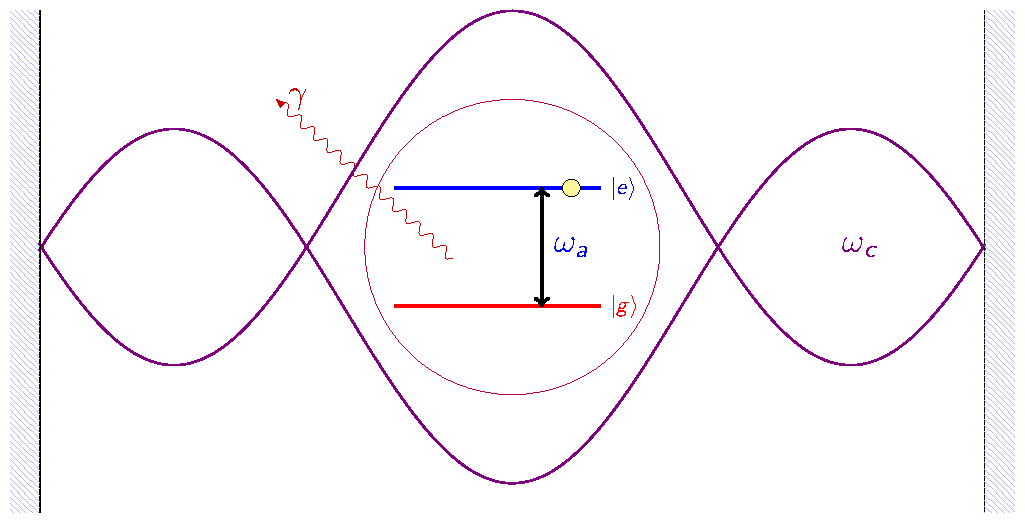
\includegraphics[width=0.7\textwidth]{Figures/presentationI.pdf}
\caption{Sketch of the situation considered by the Hamiltonian of Jaynes-Cummings.}
\label{Jaynescummings}
\end{figure}

%%%%-------- Partial measurements----------%%%%%
\section{Partial measurement and partial trace.}\label{appendixAparcialtrace}



Density matrices were introduced by the purpose of understand how is encode all the accessible information about a quantum mechanical system. It turns out that the ``pure'' states described by vectors $\ket{\psi}$ on Hilbert space\footnote{It is always possible to find a vector representation for a given quantum system. This can be done via the Gelfand-Neumark-Segal construction.}, are idealised descriptions that cannot characterize statistical mixtures which often occur in nature.  
Let's consider two systems $A$, $B$, with associate Hilbert spaces $\mathcal{H}_A$ and $\mathcal{H}_B$ respectively. If the state of the joint system $AB$ with Hilbert space $\mathcal{H}=\mathcal{H}_A\otimes\mathcal{H}_B$ is pure then it is possible that the states of $A$ and $B$ are not themselves pure. However, if there is a density matrix $\rho_{AB}$ that describes the joint state of these systems then we should be able to define density matrices for the individual systems.In fact for any observable $X:\mathcal{H}\rightarrow\mathcal{H}_{i}$, with $\mathcal{H}_{i}\subset\mathcal{H}$, $A$ or $B$ should have well-defined expectation value, and this can be used to define a reduced matrix for the system $A$ or $B$. Mathematically we denote the density matrix of system $A$ by $\rho_A$, and this matrix has to satisfy:
\begin{equation}
\text{tr}[\rho_AX]=\text{tr}[\rho_{AB}(X\otimes\mathds{1}).]
\label{partialdensitymatrix}
\end{equation}
One can proof that this density matrix is unique and always exist. similarly we can define the state of the system $B$ to be $\rho_B$ by satisfying $\text{tr}[\rho_BX]=\text{tr}[\rho_{AB}(\mathds{1}\otimes X)]$.\\
Writing explicitly  \eqref{partialdensitymatrix}:
\[
\sum_{a,a'}\rho_{A,a,a'}X_{a,a'}=\sum_{a,b,a',b'}
\rho_{AB,ab,a'b'}X_{a,a'}\delta_{b,b'}=\sum_{a,a',b}
\rho_{AB,ab,a'b}X_{a,a'}.
\]
Since this should be valid for any observable $X$ we get:
\[\rho_{A}=(\text{tr}_B[\rho])_{a,a'}=\sum_b\rho_{AB,ab,a'b}.\]

So from this result it seems like if we take the trace over $B$ while leaving $A$ alone we can compute the expression in  \eqref{partialdensitymatrix}. From the latter result we can see that the \textit{partial trace} is a map $\mathcal{L}$ such that: $\mathcal{L}_{B}(\mathcal{H})\rightarrow\mathcal{H}_{A}$ for the case of taking the trace over $B$, and we can compute the density matrix as: $\rho_{A}=\text{tr}_{B}[\rho_{AB}]$. The partial trace is the quantum analogue of the rule for marginals of probability distributions: $p_{X}(x)=\sum_{y}p_{XY}(x,y)$.\\
A similar equation holds for 
$\rho_B\equiv\text{tr}_B[\rho_{AB}]$
 which can be expressed in terms of matrix elements as
\[
\rho_{B,b,b'}=(\text{tr}[\rho])_{b,b'}=\sum_a\rho_{AB,ab,ab'}.
\]

To illustrate in a better way the way we can compute this partial trace, let's see the example of spontaneous emission from \ref{spontaneous emission}.
\[
\ket{\psi}=e{\frac{i}{\hbar}\hat{H}t}\frac{\ket{g}+\ket{e}}{\sqrt{2}}\otimes\ket{0}.
\]
With $\hat{H}=\Omega(\ket{g}\bra{e}\otimes\hat{a}^{\dagger}+\ket{e}\bra{g}\otimes\hat{a}$. $\hat{H}\ket{g,0}=0$ and $\hat{H}$ acts on the $\{\ket{e,0},\ket{g,1}\}$ subspace as a rotation. Thus:
\[
\rho=\ket{\psi}\bra{\psi}=\bordermatrix{~&\bra{g,0}&\bra{e,0}&\bra{g,1}&\bra{e,1}\cr
			\ket{g,0}&\frac{1}{2} & \frac{1}{2}\cos\theta & \frac{i}{2}\sin\theta & 0\cr
			\ket{e,0}&\frac{1}{2}\cos\theta & \frac{1}{2}\cos^2\theta & \frac{i}{2}\cos\theta\sin\theta & 0\cr
			\ket{g,1}&-\frac{i}{2}\sin\theta & -\frac{i}{2}\sin\theta\cos\theta & \frac{1}{2}\sin^2\theta & 0\cr
			\ket{e,1}&0 & 0 & 0 & 0\cr}
\]
The reduced state of the atom is
\[
\text{tr}_{photon}\ket{\psi}\bra{\psi}=
\bordermatrix{~&\bra{g}&\bra{e}\cr
			\ket{g}&\frac{1}{2}+\frac{1}{2}\sin^2\theta & \frac{1}{2}\cos\theta\cr
			\ket{e}&\frac{1}{2}\cos\theta & \frac{1}{2}\cos^2\theta\cr},
\]

and the reduced state of the photon is:

\[
\text{tr}_{atom}\ket{\psi}\bra{\psi}=\bordermatrix{~&\bra{0}&\bra{1}\cr
			\ket{0}&\frac{1}{2}+\frac{1}{2}\cos^2\theta & \frac{i}{2}\sin\theta\cr
			\ket{1}&-\frac{i}{2}\sin\theta & \frac{1}{2}\sin^2\theta\cr}.
\]
%%%%-------- Interaction picture----------%%%%%
\chapter{The Interaction Picture.}\label{appendixBinteractionpicture}

Sometimes express the operators and states in other equivalent representation or ``picture'' is of great importance in solving problems in quantum mechanics in a perturbative fashion.
We begin by considering a Hamiltonian of the form:
\begin{equation}
\hat{H}=\hat{H}_0 +\hat{V}.
\label{eq1interaction}
\end{equation}
Here $\hat{H}_0$ denotes the part of the Hamiltonian that describes the free or unperturbed evolution of the system $\mathcal{S}$, whereas $\hat{V}$ is some added external perturbation. From standard quantum theory, we know that the expectation value of an operator observable $\hat{A}(t)$ is given by the trace as in \eqref{appendixexpectedvalue}.
\begin{equation}
\braket{\hat{A}(t)}=\text{tr}\left[\hat{A}(t)\rho(t)\right]=\text{tr}\left[\hat{A}(t)e^{-\frac{i}{\hbar}\hat{H}t}\rho(0)e^{\frac{i}{\hbar}\hat{H}t}\right].
\label{eq2interactionpicture}
\end{equation}
But by using the fact that the trace is invariant under cyclic permutations of the arguments ($\text{tr}(\hat{A}\hat{B}\hat{C}\ldots)=\text{tr}(\hat{B}\hat{C}\ldots\hat{A})$) the expected value of $\hat{A}$ can be written as:
\begin{equation}
\braket{\hat{A}(t)}=\text{tr}\left[\left(e^{\frac{i}{\hbar}\hat{H}_0 t}\hat{A}(t)e^{-\frac{i}{\hbar}\hat{H}_0 t}\right)\left(e^{\frac{i}{\hbar}\hat{H}_0 t}e^{-\frac{i}{\hbar}\hat{H}t}\rho(0)e^{\frac{i}{\hbar}\hat{H}t}e^{-\frac{i}{\hbar}\hat{H}_0t}\right)\right].
\label{eq3interactionpicture}
\end{equation}
Equation  \eqref{eq3interactionpicture} take us to now introduce the \textit{interaction-picture}form of general operators $\hat{A}(t)$ and density matrices $\rho(t)$ as:
\begin{equation}
\hat{A}_I(t)=e^{\frac{i}{\hbar}\hat{H}_0t}\hat{A}(t)e^{-\frac{i}{\hbar}\hat{H}_0t},
\label{eq4interactionpicture}
\end{equation}
\begin{align}
\label{eq5interactionpicture}
\begin{split}
\rho_I(t)&=e^{\frac{i}{\hbar}\hat{H}_0t}\rho(t)e^{-\frac{i}{\hbar}\hat{H}_0t}
\\
&=e^{\frac{i}{\hbar}\hat{H}_0t}e^{-\frac{i}{\hbar}\hat{H}t}\rho(0)e^{\frac{i}{\hbar}\hat{H}t}e^{-\frac{i}{\hbar}\hat{H}_0t}.
\end{split}
\end{align}
Here the subscript $I$ is used to refer interaction-picture operator. As we note, the dynamics in the interaction-picture is determined by the  Hamiltonian ($\hat{H}_0$) instead of the total Hamiltonian ($\hat{H}$). Hence with equations \eqref{eq4interactionpicture} and \eqref{eq5interactionpicture} the expected value can be written as:
\begin{equation}
\braket{\hat{A}(t)}=\text{tr}(\hat{A}_I(t)\rho_I(t)).
\label{eq6interactionpicture}
\end{equation}
Now we would like to know the evolution of the interaction-picture density matrix $\rho_I(t)$, and to do so we use the equation \eqref{liouville-vonnuemann} to obtain:
\begin{align}
i\hbar\frac{d}{dt}\rho_I(t)&=-[\hat{H}_0,\rho_I(t)]+e^{\frac{i}{\hbar}\hat{H}_0t}\left(i\hbar\frac{d}{dt}\rho(t)\right)e^{-\frac{i}{\hbar}\hat{H}_0t}\nonumber\\
&=-[\hat{H}_0,\rho_I(t)]+e^{\frac{i}{\hbar}\hat{H}_0t}[\hat{H},\rho(t)]e^{-\frac{i}{\hbar}\hat{H}_0t}\nonumber\\
&=-[\hat{H}_0,\rho_I(t)]+e^{\frac{i}{\hbar}\hat{H}_0t}[\hat{H}_0+\hat{V},\rho(t)]e^{-\frac{i}{\hbar}\hat{H}_0t}\nonumber\\
&=-[\hat{H}_0,\rho_I(t)]+[\hat{H}_0,\rho_I(t)]+[\hat{V}_I,\rho_I(t)]\nonumber\\
&=[\hat{V}_I(t),\rho_I(t).]
\label{eq7interactionpicture}
\end{align}
This establishes the first main result:
\begin{itemize}
\item The time evolution of the interaction-picture density operator is given by an equation of the Liouville-von Neumann kind, but with the interaction-picture perturvation ($\hat{V}_I(t)$) instead of the full Hamiltonian $\hat{H}$.
\end{itemize}
 The equation \eqref{eq7interactionpicture} is often refereed as \textit{interaction-picture Liouville-von Neumann equation}.\\
Until now, we have considered the case of one system $\mathcal{S}$ subject to some perturbation $\hat{V}$ whose origin was not specified further. Let's suppose that the perturbation is due to the interaction with some external environment $\mathcal{E}$ described by an interaction Hamiltonian ($\hat{H}_{int}\equiv \hat{V}$). Denoting the Hamiltonians of the system and the environment as $\hat{H}_{\mathcal{S}}$ and $\hat{H}_{\mathcal{E}}$ respectively. Then the total Hamiltonian of the composite system $\mathcal{SE}$ can be written as:
\[
\hat{H}=\hat{H}_0+\hat{V}\equiv\overbrace{\hat{H}_{\mathcal{S}}+\hat{H}_{\mathcal{E}}}^{\equiv\hat{H}_0}+\underbrace{\hat{H}_{int}}_{\equiv \hat{V}}.
\] 
As before, we are interested in determining the time evolution of the reduce density operator $\rho_{\mathcal{S}}^{(I)}(t)$\footnote{Here the super index refers to the representation in the interaction picture.}. But as we mentioned before, in order to get information about the system, we would like to obtain the reduced interaction-picture density operator
\[
 \rho_{\mathcal{S}}^{(I)}(t)\equiv\text{tr}_{\mathcal{E}}[\rho_{I}(t)].
\]
Evaluating this last term we get:
\begin{align}
\text{tr}_{\mathcal{E}}[\rho^{(I)}(t)]&=\text{tr}_{\mathcal{E}}\left[e^{\frac{i}{\hbar}\hat{H}_0t}\rho(t)e^{-\frac{i}{\hbar}\hat{H}_0t}\right]\nonumber\\
&=e^{\frac{i}{\hbar}\hat{H}_{\mathcal{S}}t}\text{tr}_{\mathcal{E}}\left[e^{\frac{i}{\hbar}\hat{H}_{\mathcal{E}}t}\rho(t)e^{-\frac{i}{\hbar}\hat{H}_{\mathcal{E}}t}\right]e^{-\frac{i}{\hbar}\hat{H}_{\mathcal{S}}t}\nonumber \\
&=e^{\frac{i}{\hbar}\hat{H}_{\mathcal{S}}t}\text{tr}_{\mathcal{E}}[\rho(t)]e^{-\frac{i}{\hbar}\hat{H}_{\mathcal{S}}t}\nonumber \\
&=e^{\frac{i}{\hbar}\hat{H}_{\mathcal{S}}t}\rho_{\mathcal{S}}(t)e^{-\frac{i}{\hbar}\hat{H}_{\mathcal{S}}t}\nonumber \\
&=\rho^{(I)}_{\mathcal{S}}(t).
\label{eq8interactionpicture}
\end{align}
The equation \eqref{eq8interactionpicture} shows that the density operator in the interaction picture is obtained by a unitary transformation of the reduced density operator in the Schr{\"o}dinger picture involving the free system Hamiltonian $\hat{H}_\mathcal{S}$.
\begin{equation}
\rho_{\mathcal{S}}^{(I)}=e^{\frac{i}{\hbar}\hat{H}_{\mathcal{S}}t}\rho_{\mathcal{S}}e^{-\frac{i}{\hbar}\hat{H}_{\mathcal{S}}t}.
\label{eq9interactionpicture}
\end{equation}
In each case the, the transformation involves only the \textit{free} Hamiltonian which only consider the contribution of System Hamiltonian. Also with the last definition given in \eqref{eq9interactionpicture} we can assure that the expectation values of an observable 
$\hat{A}_{\mathcal{S}}(t)$ are the same in Schr{\"o}dinger picture as well as in the interaction picture\footnote{The proof of \eqref{eq10interactionpicture} can be done easily by replacing on the definition of $\hat{A}_{\mathcal{S}}^{(I)}$.
\[
\text{tr}_{\mathcal{S}}\left[\rho_{\mathcal{S}}^{(I)}\hat{A}_{\mathcal{S}}^{(I)}(t)\right]=\text{tr}_{\mathcal{S}}\left[e^{\frac{i}{\hbar}\hat{H}_{\mathcal{S}}t}\rho_{\mathcal{S}}(t)e^{-\frac{i}{\hbar}\hat{H}_{\mathcal{S}}t}e^{\frac{i}{\hbar}\hat{H}_{\mathcal{S}}t}\hat{A}_{\mathcal{S}}(t)e^{-\frac{i}{\hbar}\hat{H}_{\mathcal{S}}t}\right]=\text{tr}_{\mathcal{S}}\left[\rho_{\mathcal{S}}(t)\hat{A}_{\mathcal{S}}(t)e^{-\frac{i}{\hbar}\hat{H}_{\mathcal{S}}t}e^{\frac{i}{\hbar}\hat{H}_{\mathcal{S}}t}\right]=\text{tr}_{\mathcal{S}}\left[\rho_{\mathcal{S}}(t)\hat{A}_{\mathcal{S}}(t)\right].
\]
}
\begin{equation}
\braket{\hat{\mathcal{S}}(t)}=\text{tr}_{\mathcal{S}}\left[\rho_{\mathcal{S}}(t)\hat{A}_{\mathcal{S}}(t)\right]=\text{tr}_{\mathcal{S}}\left[\rho_{\mathcal{S}}^{(I)}(t)\hat{A}_{\mathcal{S}}^{(I)}(t)\right].
\label{eq10interactionpicture}
\end{equation}
Finally we are interested in the time evolution of the operator $\rho_{\mathcal{S}}^{(I)}(t)$, for this we take the equation \eqref{eq7interactionpicture} and we trace in both sides over the environment and then use the equation \eqref{eq8interactionpicture}, with $\hat{V}_I(t)\equiv\hat{H}_{int}^{(I)}(t)$, yields,
\begin{equation}
i\hbar\frac{d}{dt}\rho_{\mathcal{S}}^{(I)}=\text{tr}_{\mathcal{E}}\left[\hat{H}_{int}^{(I)}(t),\rho^{(I)}(t)\right].
\label{eq11interactionpicture}
\end{equation}
Looking thoroughly at this equation we can say that this equation is not of the standard \textit{Liouville-Von Neumann} form , since the right hand side depends on the total density operator $\rho^{(I)}(t)$ instead of the reduced operator $\rho^{(I)}_{\mathcal{S}}$. This is not too surprising because the state of the environment will generally influence the evolution of the reduced density operator.\\
Therefore in general, it's necessary to consider the full interacting system-environment combination to determine the reduced dynamics. This result is of course independent if we work in the Scr{\o"}dinger or the interaction picture. 
  
%\chapter{Observables y Probabilidades en el Espacio de Fase}\label{ch:observablesfs}
%\textcolor{red}{Acá puse de forma explícita los cálculos para un par de relaciones que puse en la parte de arriba, me parece que en el texto es más importante interpretar y tratar de dejar ideas claras que hacer las cuentas, total también me parece bueno verlas y por eso las pongo acá.}
\chapter{Superoperators.}\label{superoperators}
A superoperator $\mathcal{J}$ is an operator on the space of Hilbert-space operator, which means that this takes an operator into another operator and is defined as
\begin{equation}
\hat{A}\rightarrow\hat{A}'=\mathcal{J}[\hat{A}].
\label{superoperatoreq1}
\end{equation}
A superoperator $\mathcal{J}$, define a quantum operator describing the time evolution of a density matrix as a map $\mathcal{J}:\rho\rightarrow\rho'$, $\rho(t)=\mathcal{J}[\rho(0)]$ , such that satisfies some properties
\begin{enumerate}
\item \textbf{Linearity:} Even though, a non-linear mapping could take a density matrix to another density matrix, by imposing linearity it is possible to arrive to results that have physical meaning. Contritely, by imposing the linearity we get that the ensemble interpretation of the density matrix  still holds. What we mean by this is basically that if have a density matrix given by $\rho=p\rho_{1}+(1-p)\rho_{2}$, which is that there is a probability $p$ for the system to be in the state $\rho_{1}$ and a with a probability $1-p$ the system is in $\rho_{2}$. then, if our map is linear he have that the probability for the system to be in the state $\rho_{1}$ and $\rho_{2}$ remains invariant 
\[\rho(t)=\mathcal{J}[\rho]=p\mathcal{J}[\rho_{1}]+(1-p)\mathcal{J}[\rho_2]=p\rho_1(t)+(1-p)\rho_2(t).\]
The latter condition is also known as a convex linear map on operators.
\item \textbf{Trace preserving and hermiticity:}  As the density matrix itself has some properties such as $0\leq\text{tr}\rho\leq 1$ and $\rho=\rho^{\dagger}$, then, we would like that the map also preserves these properties, this is the reason why we have to impose $0\leq \text{tr} \mathcal{J}[\rho]\leq 1$, as the map could also describe a non-unitary evolution, we must normalise the map $\rho(t)\rightarrow\rho(t)/\text{tr}[\rho(t)]$. The condition of hermiticity should be also satisfy $\mathcal{J}\rho=\left[\mathcal{J}\rho\right]^{\dagger}$.
\item \textbf{Complete positivity:} This property means that the map is such that $\mathcal{J}[\rho]$ is non-negative for any extension of a Hilbert space. This can be interpreted  in a bipartite system as if we have a map that acts on the system 1 $\mathcal{J}_{1}$ and we apply it, we require that $\mathcal{M}_{1}\otimes\mathbb{I}_{2}$ is also positive for any extension of the first Hilbert space.
\end{enumerate}
If a superoperator fulfils the conditions of linearity, trace preserving, Hermiticity preservation and complete positivity, the kraus representation theorem gives us a way to write explicitly the map.
\subsection*{Kraus representation theorem.}
A map $\mathcal{J}_{A\rightarrow B}$ from a finite-dimensional Hilbert space $\mathcal{H}_{A}$ to a finite-dimensional Hilbert space $\mathcal{H}_{B}$ is linear, completely positive and trace-preserving if and only if it has a Kraus decomposition (representation) as follows\cite{Kraus}
\begin{equation}
\mathcal{J}_{A\rightarrow B}(\rho_{A})=\sum_{j}\hat{K}_{j}\rho_{A}\hat{K}_{j}^{\dagger},
\label{Kraustheorem}
\end{equation} 
where $\rho_{A}:\mathcal{H}_{A}\rightarrow\mathcal{H}_{A}$, $\hat{K}:\mathcal{H}_{A}\rightarrow\mathcal{H}_{B}$ for all $j\in \{0,...,d-1\}$,
\begin{equation}
\sum_{j}\hat{K}_{j}^{\dagger}\hat{K}_{j}=\mathbb{I}_{A},
\label{Krauscompleteness}
\end{equation}
and $d\leq\text{dim}(\mathcal{H}_{A})\text{dim}(\mathcal{H}_{B})$.
%%%%%%%%%%%%%%%%%%%%%------------------------------------------------------%%%%%%%%%%%%%%
\chapter{Lindblad equation}\label{Lindbladappendix}
A quantum system which is weakly coupled to its environment and the state of the environment does not feel or does not change significantly due to the interaction with the environment can be treated via Born-Markov Master equation, this leads us to a Markovial evolution for the reduced density matrix $\rho$ of the system, and the most general form of the quantum master equation such that the positivity of the density matrix is assured is know as Lindblad equation\footnote{Here $\{..\}_{+}$ denotes the anticommutator. }
\begin{equation}
\dot{\rho}=\mathcal{L}\rho=-\frac{i}{\hbar}[\hat{H},\rho]+\sum_{k}\hat{J}_{k}\rho\hat{J}_{k}^{\dagger}-\frac{1}{2}\{\hat{J}^{\dagger}_{k}\hat{J}_{k},\rho\}_{-},
\label{Lindblad1}
\end{equation} 
where $\{\hat{J}_{k}\}_{k=1}^{K}$ is the set of Lindblad operators, these operators as we said before describe the coupling between the system and the reservoir. However, the representation of \eqref{Lindblad1} is not unique, therefore, we have the freedom to redefine the Lindblad operators by an arbitrary $K\times K$ unitary matrix $T_{kl}$\cite{0305-4470-26-9-019}.
\begin{equation}
\hat{J}_{k}\rightarrow\hat{J}_{l}=\sum_{k}T_{lk}\hat{J}_{k}\Rightarrow \hat{J}_{k}=\sum_{l}T_{lk}^{\dagger}\hat{J}_{l},
\label{Lindblad2}
\end{equation} 
as we required that the matrix has to be unitary
\[\sum_{k}T_{kl}T^{\dagger}_{kl'}=\delta_{ll'},\]
using this relation it is possible to check that the equation \eqref{Lindblad1} stays invariant under these transformations,
\begin{align}
\dot{\rho}=&=-\frac{i}{\hbar}[\hat{H},\rho]+\sum_{ljk}\left(\underbrace{T{\dagger}_{lk}T_{jk}}_{\delta_{lj}}\hat{J}_{l}\rho\hat{J}_{j}^{\dagger}-\frac{1}{2}\{\hat{J}^{\dagger}_{l}\underbrace{T_{lk}T_{jk}{\dagger}}_{\delta_{lj}}\hat{J}_{j},\rho\}\right)\nonumber\\
&=-\frac{i}{\hbar}[\hat{H},\rho]+\sum_{l}\hat{J}_{l}\rho\hat{J}_{l}^{\dagger}-\frac{1}{2}\{\hat{J}^{\dagger}_{l}\hat{J}_{l},\rho\}_{-},\label{Lindblad3}
\end{align} 

which has the same form of \eqref{Lindblad1}, so, Lindblad equation is invariant under unitary transformations over the operators.\\
Other interesting property that Lindblad master equation has is that is invariant under a shift on the operator $\hat{J}_{k}$ if we also change the Hamiltonian. To see how this should change consider a shift of the form
\[\hat{J}_{k}\rightarrow \hat{J}_{k}+\chi_{k}*\hat{\mathbb{I}},\]
where $\chi_{k}$ is a complex number, and the Hamiltonian should change as
\[\hat{H}\rightarrow \hat{H}-\frac{i\hbar}{2}(\chi^{*}_{k}\hat{J}_{k}-\chi_{k}\hat{J}_{k}^{\dagger}).\]
So, inserting this expressions in the equation \eqref{Lindblad1} we get
\begin{equation*}
\dot{\rho}=-\frac{i}{\hbar}[\hat{H},\rho]-\frac{1}{2}[\chi_{k}^{*}\hat{J}_{k}-\chi_{k}\hat{J}^{\dagger}_{k},\rho]+\sum_{k}(\hat{J}_{k}+\chi_{k})\rho(\hat{J}^{\dagger}_{k})+\chi_{k}^{*})-\frac{1}{2}\{(\hat{J}_{k}^{\dagger}+\chi_{k}^{*})(\hat{J}_{k}+\chi_{k}),\rho\}_{-},
\end{equation*}
computing the terms inside the sum, we get 
\[
\hat{J}_{k}\rho\hat{J}_{k}^{\dagger}-\frac{1}{2}\{\hat{J}_{k}^{\dagger}\hat{J}_{k},\rho\}_{-}+\cancel{\chi^{*}_{k}\hat{J}_{k}\rho}+\cancel{\chi_{k}\rho\hat{J}^{\dagger}_{k}}+\cancel{\chi^{2}_{k}\rho}
-\frac{1}{2}\chi_{k}\hat{J}_{k}^{\dagger}\rho-\cancel{\frac{1}{2}\chi_{k}\rho\hat{J}^{\dagger}_{k}}-\cancel{\frac{1}{2}\chi^{*}_{k}\hat{J}_{k}\rho}
-\frac{1}{2}\chi^{*}_{k}\rho\hat{J}_{k}-\cancel{\chi^{2}_{k}\rho}
\]
\begin{equation}
=\hat{J}_{k}\rho\hat{J}_{k}^{\dagger}-\frac{1}{2}\{\hat{J}_{k}^{\dagger}\hat{J}_{k},\rho\}_{-}+\frac{1}{2}\chi^{*}_{k}\hat{J}_{k}\rho+\frac{1}{2}\chi_{k}\rho\hat{J}^{\dagger}_{k}-\frac{1}{2}\chi_{k}\hat{J}_{k}^{\dagger}\rho-\frac{1}{2}\chi^{*}_{k}\rho\hat{J}_{k}.\label{firsttermsum}
\end{equation}
Computing the commutator
\begin{equation}
-\frac{1}{2}[\chi_{k}^{*}\hat{J}_{k}-\chi_{k}\hat{J}_{k}^{\dagger},\rho]=\-\frac{1}{2}\chi^{*}\hat{J}_{k}\rho+\frac{1}{2}\chi^{*}\rho\hat{J}_{k}+\frac{1}{2}\chi_{k}\hat{J}_{k}^{\dagger}\rho-\frac{1}{2}\chi_{k}\rho\hat{J}_{k}^{\dagger},
\label{commutator}
\end{equation}
combining \eqref{firsttermsum} and \eqref{commutator} it leads us to
\begin{equation}
\dot{\rho}=-\frac{i}{\hbar}[\hat{H},\rho]+\sum_{k}\hat{J}_{k}\rho\hat{J}^{\dagger}_{k}-\frac{1}{2}\{\hat{J}^{\dagger}_{k}\hat{J}_{k},\rho\}_{-}.\label{Lindblad4}
\end{equation}
Then from the result given in \eqref{Lindblad4} wee see that Lindblad equation is invariant under shifts.\\
The last interesting property of Lindblad equation is its invariance under gauge transformations over the state
\begin{equation}
\ket{\psi(t)}\rightarrow\ket{\phi}=\text{exp}\left[\frac{i}{\hbar}\chi(t)\right]\ket{\psi(t)},
\label{Lindblad5}
\end{equation}
where $\chi(t)$ is an arbitrary function of time, this is know as a \textit{gauge transformation} and does not have any effect on any physical properties of the system, since all observables and the density matrix would change as.
\begin{align}
\braket{\hat{O}}\rightarrow\braket{\hat{O}'}&=\bra{\phi}\hat{O}\ket{\phi}=\bra{\psi(t)}e^{-\frac{i}{\hbar}\chi(t)}\hat{O}e^{\frac{i}{\hbar}\chi(t)}\ket{\psi(t)}=\braket{\hat{O}},\\
\rho\rightarrow\rho'&=\ket{\phi}\bra{\phi}=e^{\frac{i}{\hbar}\chi(t)}\ket{\psi(t)}\bra{\psi(t)}e^{-\frac{i}{\hbar}\chi(t)}=\rho.
\end{align}




\end{appendix}